\chapter{Pruebas}

	\noindent En este capítulo se presentará una breve descripción acerca de las pruebas realizadas de tal manera este sea comprobado que tiene garantía. \\
	
	\noindent De tal manera, las pruebas se realizaron con base a Clases de Equivalencia. En la cual se se plantean los posibles casos que se pueden llegar a presentar en un módulo. Estos casos se crean o toman con base en el caso de uso correspondiente, es decir, por cada caso de uso que se tiene en el sistema debe existir un guión de prueba.\\
	
	\noindent La ventaja con este tipo de pruebas es que nos permite cubrir todos los posibles escenarios en un módulo en específico. Para saber el número de pruebas que son necesarias realizar se debe seguir la siguiente formula matemática:\\
	$ n1 * n2 * ... * n_{n} $ \\
	donde, 
	n, corresponde al número de entradas que tiene el caso de uso.\\
	n1, este valor corresponde al número de pruebas que se realicen en cada uno de las entradas del caso de uso.\\
	
	\noindent Ahora bien, hay otra formula la cual indica el número de pruebas minímas necesarías para considerar que el caso de uso analizando tiene cálidad, la formula matemática es la siguiente: \\
	
	$ (n1 + n2 + ... + n_{n}) - (n - 1) $
	
	n, corresponde al número de entradas que tiene el caso de uso.\\
	n1, este valor corresponde al número de pruebas que se realicen en cada uno de las entradas del caso de uso.\\
	
	\noindent Tomando en cuenta lo antes mencionado, se realizaron las pruebas correspondientes, a continuación se mostrarán los guiónes de prueba de alguno de los módulos representativos de la aplicación web.\\
	\pagebreak
	
	\textbf{Guión de prueba del caso de uso 10: Agrega resultados}
	
	\begin{figure}[hbt!]
		\centering
		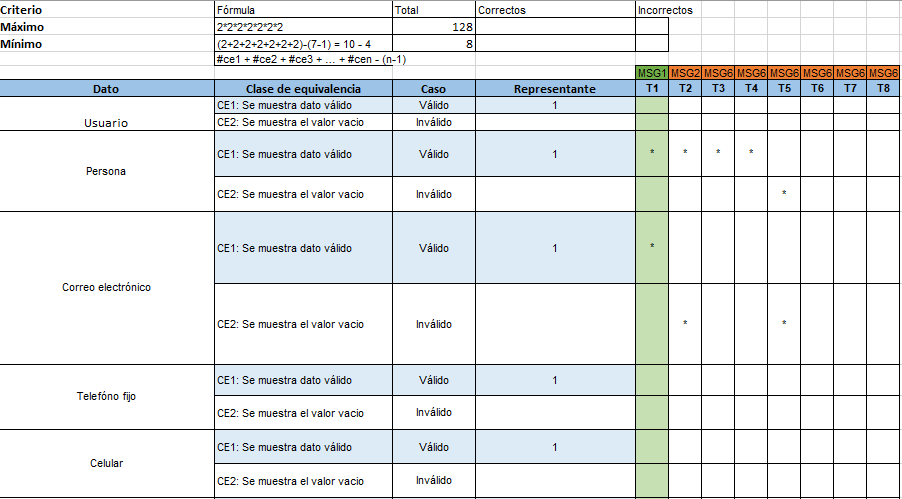
\includegraphics[width=14cm, height=6cm]{Imagenes/Pruebas/GuionPruebaCU10}
		\caption{Tabla correspondiente al guión de prueba del caso de uso 10}
		\label{guionpruebaCU10}
	\end{figure}

	\textbf{Guión de prueba del caso de uso 11: Agrega resultados}

	\begin{figure}[hbt!]
		\centering
		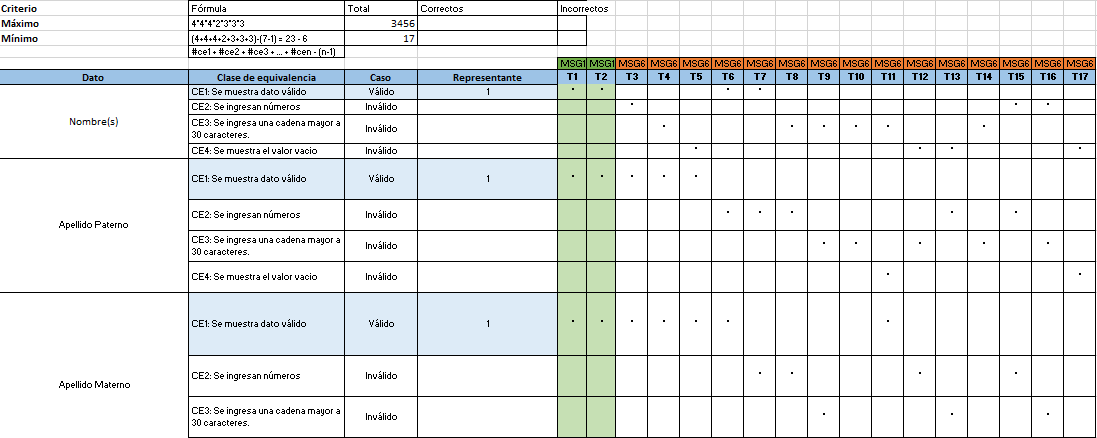
\includegraphics[width=14cm, height=6cm]{Imagenes/Pruebas/GuionPruebaCU11}
		\caption{Tabla correspondiente al guión correspondiente al CU11}
		\label{guionpruebaCU11}
	\end{figure}
\pagebreak

	\textbf{Guión de prueba del caso de uso 11: Agrega resultados}
	\begin{figure}[hbt!]
		\centering
		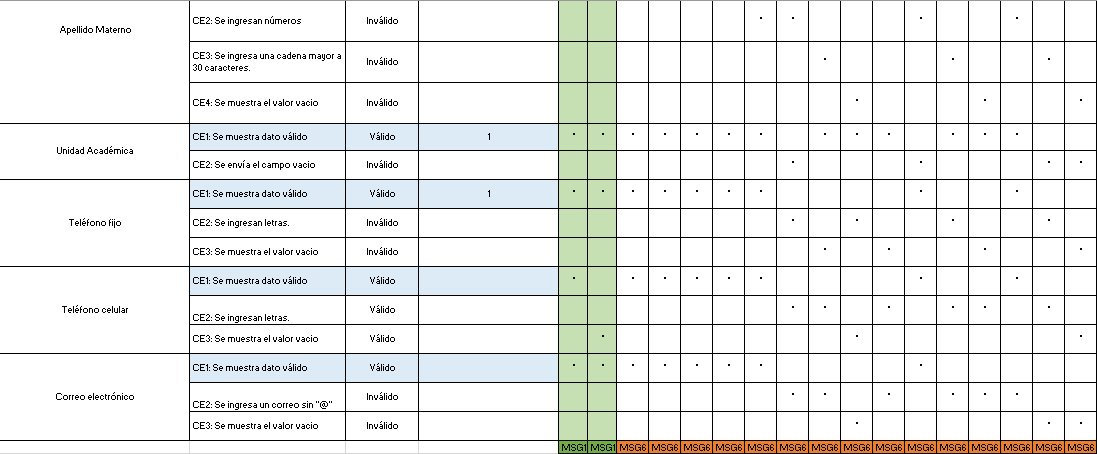
\includegraphics[width=14cm, height=6cm]{Imagenes/Pruebas/GuionPruebaCU11_1}
		\caption{Tabla correspondiente al guión correspondiente al CU11}
		\label{guionpruebaCU11_1}
	\end{figure}

	\textbf{Guión de prueba del caso de uso 15: Agrega resultados}
	\begin{figure}[hbt!]
		\centering
		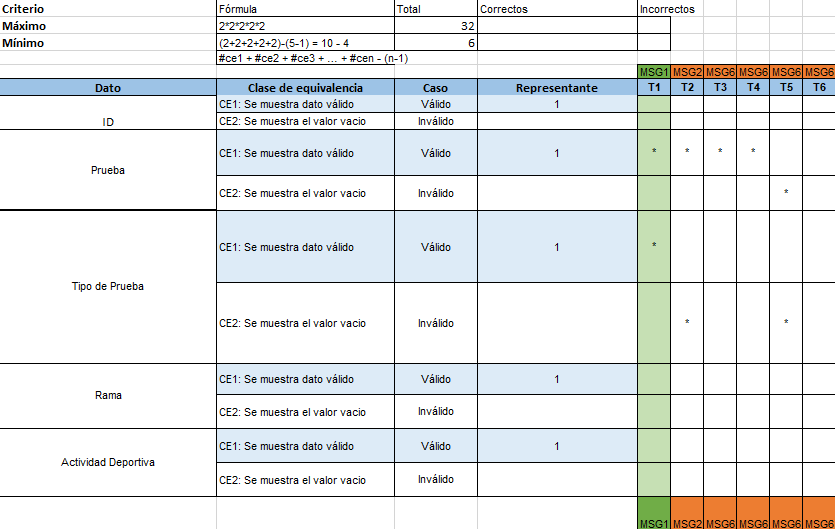
\includegraphics[width=14cm, height=6cm]{Imagenes/Pruebas/GuionPruebaCU15}
		\caption{Tabla correspondiente al guión correspondiente al CU15}
		\label{guionpruebaCU15}
	\end{figure}
\pagebreak
	
	\textbf{Guión de prueba del caso de uso 16: Agrega resultados}	
	\begin{figure}[hbt!]
		\centering
		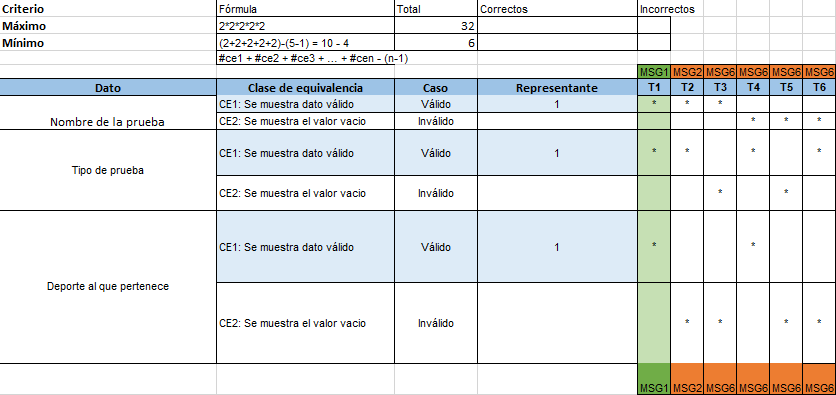
\includegraphics[width=14cm, height=6cm]{Imagenes/Pruebas/GuionPruebaCU16}
		\caption{Tabla correspondiente al guión correspondiente al CU16}
		\label{guionpruebaCU16}
	\end{figure}
	
	\textbf{Guión de prueba del caso de uso 22: Agrega resultados}	
	\begin{figure}[hbt!]
		\centering
		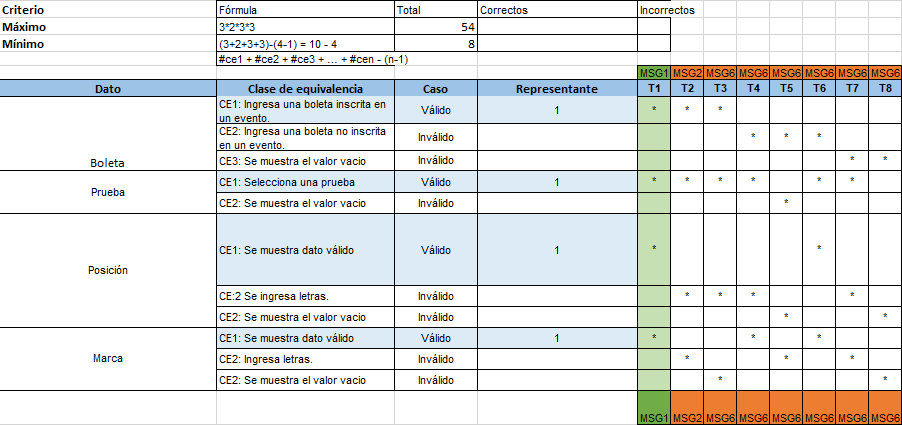
\includegraphics[width=14cm, height=6cm]{Imagenes/Pruebas/GuionPruebaCU22}
		\caption{Tabla correspondiente al guión correspondiente al CU22}
		\label{guionpruebaCU22}
	\end{figure}
	
	
	